\documentclass{beamer}
\usepackage[utf8]{inputenc}
\usetheme{Madrid}
\usecolortheme{default}

% math & fonts
\usepackage{amsmath,amssymb,amsthm}
\usepackage{txfonts}
\usepackage{lmodern}

% drawing / figures / listings
\usepackage{tkz-euclide}
\usepackage{tikz}
\usepackage{graphicx}
\usepackage{listings}
\usepackage{xcolor}
\usepackage{array}
\usepackage{tabularx}
\usepackage{adjustbox}

% (optional) your local package; comment if not available
\usepackage{gvv}

% vector macro
\newcommand{\myvec}[1]{\begin{bmatrix}#1\end{bmatrix}}

% show total frame count in footer
\setbeamertemplate{page number in head/foot}[totalframenumber]

% listing defaults
\lstset{
    language=C,
    basicstyle=\ttfamily\small,
    keywordstyle=\color{blue},
    stringstyle=\color{orange},
    commentstyle=\color{green!60!black},
    numbers=left,
    numberstyle=\tiny\color{gray},
    breaklines=true,
    showstringspaces=false,
}

\title{Matgeo-q.4.13.1}
\author{AI25BTECH11036-SNEHAMRUDULA}
\date{\today}

\begin{document}

\begin{frame}
  \titlepage
\end{frame}

\section{Question}
\begin{frame}{Question}
Consider the lines
\[
\begin{aligned}
L_1 &: x + 3y - 5 = 0, \\
L_2 &: 3x - ky - 1 = 0, \\
L_3 &: 5x + 2y - 12 = 0.
\end{aligned}
\]
Match the statements in Column I with Column II (choices refer to values of \(k\) or relations).
\begin{center}
\begin{tabular}{p{0.45\linewidth} p{0.45\linewidth}}
\textbf{Column I} & \textbf{Column II} \\
\begin{enumerate}[label=(\Alph*)]
    \item $L_1, L_2, L_3$ are concurrent, if
    \item One of $L_1, L_2, L_3$ is parallel to at least one of the other two, if
    \item $L_1, L_2, L_3$ form a triangle, if
    \item $L_1, L_2, L_3$ do not form a triangle, if
\end{enumerate}
&
\begin{enumerate}[label=(\alph*)]
    \item $k = 9$
    \item $k = \dfrac{-6}{5}$
    \item $k = \dfrac{5}{6}$
    \item $k = 5$
\end{enumerate}
\end{tabular}
\end{center}
\end{frame}

\section{Solution}
\begin{frame}{Solution — (A) Concurrency}
Intersection of \(L_1\) and \(L_3\):
\[
\begin{cases}
x+3y=5,\\[4pt]
5x+2y=12,
\end{cases}
\quad\Rightarrow\quad 13y=13,\; y=1,\; x=2.
\]
So intersection point is
\[
\vec{x}_0=\myvec{2\\1}.
\]
This point lies on \(L_2\) iff
\[
\begin{aligned}
\myvec{3\\-k}^{\!\top}\myvec{2\\1}=1
&\iff 6-k=1\\
&\iff k=5.
\end{aligned}
\]
Hence the three lines are concurrent precisely when \(k=5\).
\end{frame}

\begin{frame}{Solution — (B) Parallelism}
Two lines are parallel iff their normals are proportional.

Normals of \(L_2\) and \(L_3\):
\[
\vec{n}_2=\myvec{3\\-k},\qquad \vec{n}_3=\myvec{5\\2}.
\]
If \(\vec{n}_2=\lambda\vec{n}_3\) then
\[
3=5\lambda,\quad -k=2\lambda \Rightarrow \lambda=\tfrac{3}{5},\; k=-2\lambda = -\tfrac{6}{5}.
\]
So a parallel pair (between \(L_2\) and \(L_3\)) occurs when \(k=-\dfrac{6}{5}\).
(Analogous checks show no other accidental proportionality with \(L_1\) for these \(k\).)
\end{frame}

\begin{frame}{Solution — (C) Triangle \& (D) Not a triangle}
\textbf{(C) Form a triangle:} The three lines form a triangle iff no two are parallel and they are not concurrent.  
Therefore triangle occurs when
\[
k\neq 5 \quad\text{and}\quad k\neq -\tfrac{6}{5}.
\]
(So any explicit example values like \(k=9\) or \(k=\tfrac{5}{6}\) satisfy the triangle condition.)

\medskip
\textbf{(D) Do not form a triangle:} This happens when the lines are concurrent or when a parallel pair exists. Hence
\[
\text{no triangle} \iff k=5 \quad\text{or}\quad k=-\tfrac{6}{5}.
\]
\end{frame}

\begin{frame}{Final concise matching}
\begin{itemize}
  \item (A) Concurrency \(\iff k=5\).
  \item (B) One line parallel to another \(\iff k=-\dfrac{6}{5}\).
  \item (C) They form a triangle \(\iff k\neq 5\) and \(k\neq -\dfrac{6}{5}\). (Examples: \(k=9,\ k=\tfrac{5}{6}\).)
  \item (D) They do \emph{not} form a triangle \(\iff k=5\) or \(k=-\dfrac{6}{5}\).
\end{itemize}
\end{frame}

\begin{frame}{Graphical Representation}
\begin{center}
% placeholder figure drawn with TikZ
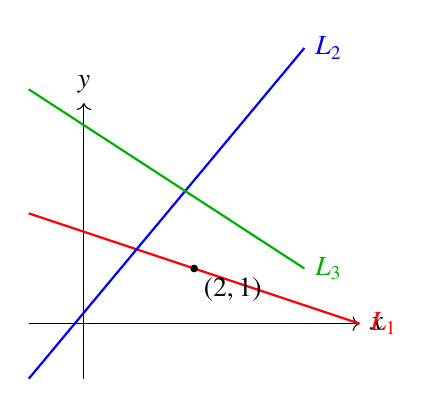
\begin{tikzpicture}[scale=0.7]
  % Axes
  \draw[->] (-1,0)--(5,0) node[right]{$x$};
  \draw[->] (0,-1)--(0,4) node[above]{$y$};

  % Lines
  \draw[red, thick] (-1,2) -- (5,0.0) node[right] {$L_1$};
  \draw[blue, thick] (-1,-1) -- (4,5) node[right] {$L_2$};
  \draw[green!70!black, thick] (-1,4.25) -- (4,1) node[right] {$L_3$};

  % Intersection point
  \fill (2,1) circle (2pt) node[below right] {$(2,1)$};
\end{tikzpicture}
\end{center}
\end{frame}

\end{document}
